% Clase del documento (class)
\documentclass[a4paper,12pt]{article}

%---------------------------------- Preámbulo del documento (preamble) ----------------------------------
\usepackage[utf8]{inputenc}
%\usepackage[latin1]{inputenc}	% Para que LATEX entienda los símbolos del teclado español.
\usepackage[T1]{fontenc}		% Para que utilice nuestros tipos acentuados.
\usepackage[spanish]{babel}		% Reglas españolas para división de sílabas, traducción de comandos, etc... 
%\usepackage{eurosym}			% Para el simbolo del euro.
%\DeclareInputText{128}{\euro}	% Para usar la tecla del euro.

\usepackage{graphicx}
\usepackage{float} 

\usepackage{url}				% Para las direcciones url
\usepackage{hyperref}			% Para hacer click en las urls en el pdf.

\usepackage[nottoc]{tocbibind}
\renewcommand\tocbibname{Referencias}

% Formato de los márgenes
%\usepackage{anysize}
%\marginsize{3cm}{3cm}{3cm}{3cm}

% Definiciones, teoremas, ... 
%\newtheorem{defi}{Definición}[section]

% Título, autor, fecha, etc.opening
\title{Anteproyecto:\\Entorno interactivo para el estudio de estrategias de IA en juegos}
\author{José Miguel Horcas Aguilera}
%\date{}

% Reglas de partición silábica.
%\hyphenation{a-tri-bu-to a-tri-bu-tos}

%------------------------------ Cuerpo del documento (document body) -----------------------------
\begin{document}

% Redefinición de comandos
%\renewcommand{\labelitemi}{$\bullet$ }
%\renewcommand{\tablename}{Tabla}

% INICIO
\maketitle			% Imprime el título, autor, fecha, etc.

\begin{abstract} 	% Resumen
\par 

\end{abstract}

\tableofcontents	% Tabla de contenidos (índice)
\clearpage

\section{Introducción}
\par 
Los juegos son un tema atractivo a estudiar para los investigadores de Inteligencia Artificial (IA).
La naturaleza abstracta de los juegos, la facilidad de representar el estado de los mismos y la definición precisa de sus reglas hace que hayan tenido mucho interés en la comunidad de IA.

\par 
Los juegos son problemas de búsqueda entre adversarios, que están ocasionados por entornos competitivos donde los objetivos de los distintos agentes están en conflicto.
Estos problemas son interesantes porque son demasiado difíciles para resolverlos.
Normalmente no es factible calcular una decisión óptima y requieren la capacidad de tomar alguna decisión \cite{RN03, N01}.

\par 
El objetivo de este proyecto es desarrollar un entorno que permita comparar el rendimiento de diferentes estrategias para juegos.
Para ello se construirá una aplicación interactiva que permita al usuario jugar y realizar pruebas con distintos agentes jugadores automáticos, generando información del rendimiento para compararlos entre sí.
Se implementará un módulo de razonamiento de un agente para juegos con un conjunto de estrategias para juegos bipersonales de suma cero e información perfecta. 
Además, se proporcionará un implementación de los juegos del Conecta-4 y del Go para comparar las estrategias.

\section{Objetivos}
\par 
El objetivo principal del proyecto es proporcionar una herramienta para el estudio de diferentes técnicas de búsqueda entre adversarios en árboles de juegos.
La aplicación permitirá jugar, realizar pruebas de rendimiento entre distintas estrategias y entrenar agentes que usen estrategias con aprendizaje.

\par 
El proyecto proporciona además un marco de trabajo para el dominio de los juegos en IA, siendo útil tanto para la docencia como para la investigación.
La aplicación se realizará sobre tecnología \textit{Java} y la documentación será un aspecto clave en este proyecto, por lo que todo el código estará documentado en formato \textit{javadoc} para que cualquier alumno, profesor o investigador pueda hacer uso de él.

\par 
La Figura~\ref{fig:sistema} muestra un esquema de la arquitectura del sistema.
Se observa la base del sistema constituida por el marco de trabajo dividido en dos partes principales relacionadas: Estrategias y Juegos, que definen las interfaces que deben implementar las estrategias y los juegos que se quieran desarrollar.
Éste incluye también el entorno de usuario interactivo y otros componentes estándar para el dominio de los juegos en IA.

\par 
Las distintas implementaciones de estrategias y juegos no forma parte del marco de trabajo, lo que permite ampliar el número de estrategias y juegos del sistema.

% Imagen
\begin{figure}[H]
\begin{center}
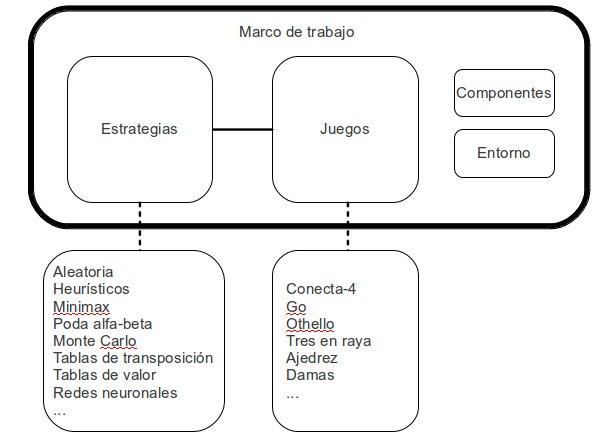
\includegraphics[scale=0.45]{sistema.jpg}
\caption{Arquitectura del sistema.}
\label{fig:sistema}
\end{center}
\end{figure}


\subsection{Estrategias}
\par 
Un agente inteligente viene definido por los siguientes elementos: unos objetivos (en el caso de los juegos el objetivo es ganar), un medio en el que se desenvuelve (por ejemplo el tablero de juego), la percepción que el agente tiene del medio, las acciones a realizar (movimiento válidos del juego) y el conocimiento que viene determinado por la estrategia usada por el agente para proponer un movimiento válido.

\par 
A continuación se exponen las principales estrategias que se implementarán y que se podrán estudiar y comparar con ayuda de la aplicación.
Se implementarán versiones generales de estas estrategias de forma que resulten sencillas de entender de cara a la docencia.
Éstas van desde el caso más básico como la estrategia aleatoria hasta algoritmos más complejos como una estrategia con aprendizaje u otra con redes neuronales, pasando por los clásicos algoritmos de evaluación minimax y poda alfa-beta, entre otros.

\par 
Además de las estrategias que se detallan a continuación, para cada juego se implementará un jugador que pida el movimiento al usuario.
De esta manera un jugador humano podrá jugar contra cualquier estrategia o incluso contra otro jugador humano.
\clearpage
\begin{itemize}
	\item \textbf{Aleatoria}\\
	La estrategia más sencilla es un agente que realice movimientos aleatorios.
%	Es interesante porque servirá de base para comparar el resto de estrategias.
	Esta estrategia además será independiente del juego en el que se use.

	\item \textbf{Evaluador heurístico}\\
	Se implementará un agente capaz de evaluar heurísticamente si una situación le es favorable o no.
	La estrategia que empleará es la siguiente: dada una situación, considerará todos los movimientos inmediatos, los evaluará heurísticamente y escogerá el mejor.
	\par 
	Esta estrategia, al contrario que la estrategia aleatoria, no se puede implementar de manera genérica, pues la función de evaluación heurística depende del tipo de juego.
	Sin embargo, se desarrollará un agente genérico el cual emplee una función de evaluación u otra en función del tipo de juego.

	\item \textbf{Minimax}\\
	El algoritmo minimax proporciona una estrategia óptima, aunque no sea factible para juegos complejos como el Go.
	Se desarrollarán varias versiones del algoritmo minimax: una con límite de profundidad en la búsqueda y otra con límite de tiempo.
	\par 
	El agente que emplee esta estrategia necesitará igualmente una función de evaluación heurística, por lo que se desarrollarán funciones de evaluación para cada juego.

	\item \textbf{Poda alfa-beta}\\
	Esta estrategia será similar a la estrategia minimax pero incluirá el algoritmo de poda alfa-beta.
	Dispondrá también de versiones con límite de profundidad en la búsqueda y con tiempo limitado.
	
	\item \textbf{Tabla de transposición}\\
	Una tabla de transposición proporciona una forma de reducir el espacio de búsqueda al considerar estados ya visitados anteriormente.
	Se desarrollará una implementación de las tablas de transposición que se incorporará a las estrategias anteriores.
%	Así podremos tener agentes que realicen búsquedas minimax aprovechando las ventajas de la tabla de transposición o agentes que realicen una búsqueda con poda alfa-beta en un tiempo limitado e incluyan una tabla de transposición.
	
	\item \textbf{Tabla de valores}\\
	Se incluirá una estrategia de aprendizaje con refuerzo empleando tablas de valor, de modo que un agente sea capaz de aprender a jugar mediante ensayo y error.
	Para ello se entrenará mediante el método de las diferencias temporales.
	
	\item \textbf{Redes neuronales}\\
	Se usará una implementación disponible de redes neuronales para construir una red neuronal capaz de evaluar los estados de los juegos \cite{JavaNN}.
	La red se entrenará mediante aprendizaje con refuerzo empleando una versión simplificada del método de las diferencias temporales.
	\par 
	El entorno interactivo dispondrá de un módulo que nos permita entrenar agentes que usen alguna de las dos estrategias anteriores.
	
	\item \textbf{Método de Monte Carlo}\\
	Se incluirá también una estrategia que incorpore una técnica estocástica, como el método de Monte Carlo para búsqueda en árboles de juegos.
	
\end{itemize}

\subsection{Juegos}
\par
El proyecto está orientado a una clase de juegos especializada: juegos de suma cero, de dos jugadores, por turnos, deterministas y de información perfecta.
Se trata de entornos deterministas, totalmente observables en los cuales hay dos agentes cuyas acciones deben alternar y en los que los valores de utilidad al final de juego son siempre iguales y opuestos; es decir, si un jugador gana, el otro necesariamente tiene que perder.

\par 
Un juego puede definirse formalmente como una clase de problemas de búsqueda que contiene: un estado inicial, una función sucesor, un test terminal y una función de utilidad o función objetivo.
Definiendo una interfaz adecuada se puede construir un módulo que permita implementar fácilmente cualquier juego del tipo considerado.

\par 
La aplicación se completará con la implementación de dos juegos que permitan ver el funcionamiento del entorno y probar las diferentes estrategias implementadas.
Estos juegos son:

\begin{itemize}
	\item \textbf{Conecta-4}\\	
	Se diseñará el clásico juego del Conecta-4 en un tablero de 6 filas por 7 columnas.
	Aunque de forma más general se tratará el juego del Conecta-K en un tablero de n x m.	
	\item \textbf{Go}\\	
	El Go es el juego de mesa más popular en Asia.
	Se juega en un tablero de tamaño 19x19, por lo que el factor de ramificación es muy elevado, comenzando en 361.
	Actualmente los computadores juegan al Go a nivel aficionado.\footnote{Recientemente se ha conseguido alcanzar el nivel \textit{master} (1 dan) en la escala de rendimiento del Go \cite{MonteCarlo}.}
	Se estudiará una versión reducida en un tablero de 9x9, aunque el juego se implementará de forma general en un tablero de n x m.
	En \cite{GameGo} puede encontrarse más información sobre el juego e investigaciones de estrategias que se han aplicado.

\end{itemize}

\subsection{Entorno interactivo de usuario}
\par 
El sistema contará con una interfaz gráfica de usuario que permita seleccionar el juego y los jugadores (estrategias a aplicar), jugar, realizar simulaciones y mostrar estadísticas para comparar las estrategias.
Además, para cada juego se desarrollará una interfaz sencilla, de forma que resulte cómodo jugar o ver el desarrollo del juego.

\subsection{Herramienta como marco de trabajo} 
\par
La herramienta proporciona un marco de trabajo (\textit{framework}) que ayuda a implementar fácilmente juegos y estrategias para juegos.
El marco de trabajo es una arquitectura especializada para el dominio de los juegos en IA.
Define un conjunto de componentes para enfocar el problema de búsquedas entre adversarios: describe las interfaces necesarias que deben implementar los juegos y estrategias; establece las reglas de interacción entre los componentes e implementa algunos componentes estándar como por ejemplo un tablero básico para los juegos que lo requieran.

\par 
Se divide en dos partes principales relacionadas: una para la representación de los juegos y otra para la especificación de las estrategias de los agentes.

\par 
El marco de trabajo sirve además como referencia para resolver nuevos problemas relacionados en el ámbito de la teoría de juegos y la inteligencia artificial.


\subsection{Aplicación para la docencia} 
\par 
La aplicación resultante del proyecto supone una herramienta novedosa y muy útil para la docencia.
Al igual que otros programas, como \cite{PathDemo} o \cite{AIDA} que muestran el funcionamiento de algoritmos de búsqueda en espacios de estados, esta nueva aplicación permite mostrar el funcionamiento de diferentes estrategias en espacios de búsqueda más complejos como son los árboles de búsqueda de los juegos.


\subsection{Aplicación para la investigación} 
\par 
La investigación en juegos ha generado varias ideas interesantes sobre cómo hacer uso, lo mejor posible, del tiempo.
Esta aplicación también supone una ayuda a la investigación en IA.
Gracias a su diseño permitirá añadir de manera cómoda otras estrategias y juegos, proporcionando información sobre la complejidad en tiempo y en espacio de cada una de las estrategias y juegos.


\section{Metodología}
\par 
Para llevar a cabo el proyecto se seguirá una metodología de desarrollo iterativa e incremental que encarezca la agilidad.
No nos decantaremos por ninguna en concreto porque el desarrollo lo realizará una sola persona.
Sin embargo, se tomarán algunas características propias de metodologías ágiles como Scrum o KanBan; por ejemplo la flexibilidad a los cambios.

\par 
Debido a las características propias del proyecto, el objetivo de aplicar una metodología de desarrollo iterativa e incremental es obtener una arquitectura robusta en las primeras etapas del proyecto que permita satisfacer los requisitos clave y poder ampliar estos requisitos evitando riesgos críticos o problemas de desarrollo que puedan surgir en posteriores fases del proyecto.

\par 
El trabajo a realizar en cada iteración se dividirá en cinco flujos de trabajo fundamentales: requisitos, análisis, diseño, implementación y prueba.
Como no todas las iteraciones serán exactamente iguales, cada iteración concreta puede pasar en mayor o menor medida por los flujos de trabajo. 
Además, la duración de las iteraciones tampoco será constante.

\par 
En la siguiente sección se muestra una planificación para el proyecto que define el trabajo a realizar en cada una de las iteraciones.


\section{Planificación del proyecto}
\par 
El proyecto se puede dividir en cuatro partes bien diferenciadas: el marco de trabajo, los juegos, las estrategias, y el entorno de usuario.
Se usará esta división para establecer las iteraciones del proyecto, las cuales se detallan a continuación.
Como se ha comentando en la sección anterior, en cada iteración se realizarán tareas de especificación, análisis, diseño, implementación y prueba.

\begin{itemize}
	\item \textbf{Primera iteración}\\
	El objetivo de la primera iteración es construir la arquitectura base del sistema, que supondrá un marco de trabajo para el desarrollo de las estrategias y de los juegos.
	Se trata de la parte más importante del proyecto y debe especificarse y diseñarse de forma robusta ya que cambios posteriores en esta parte pueden ser muy difíciles de llevar a cabo.
	
	\item \textbf{Segunda iteración}\\
	En esta segunda iteración se implementarán los juegos siguiendo las interfaces definidas en la iteración anterior.
	El hecho de desarrollar los juegos antes que las estrategias no es casual: tener desarrollado un espacio de estados concreto de un juego, nos permitirá realizar pruebas reales de las estrategias directamente conforme estas últimas se vayan desarrollando y poder corregir posibles errores en los algoritmos.
	También se definirá una estrategia que permita al usuario humano realizar un movimiento válido.
	El desarrollo de la interfaz gráfica de los juegos puede incluirse en esta iteración o dejarse para la última puesto que es indiferente para la realización de las pruebas.
	
	\item \textbf{Tercera iteración}\\
	Se estudiarán e implementarán las diferentes estrategias propuestas, incluyendo funciones heurísticas para cada juego.
	
	\item \textbf{Cuarta iteración}\\
	En la última iteración se desarrollará el entorno de usuario interactivo.
	Éste englobará las estrategias y los juegos creados, permitiendo jugar, realizar pruebas de rendimiento o entrenar jugadores, mediante una interfaz gráfica sencilla e intuitiva.
	
	
\end{itemize}

\section{Herramientas}
\par 
A continuación se exponen los métodos materiales que se usarán para llevar a cabo el proyecto.

\begin{itemize}
	\item La especificación y el diseño del proyecto se realizará en lenguaje \textbf{UML} con el programa \textbf{MagicDraw}.
	
	\item La aplicación completa se desarrollará en \textbf{Java}.
	Aunque el diseño del proyecto permite implementarlo en cualquier otro lenguaje orientado a objetos sin ninguna dificultad.
	Para el desarrollo de la interfaz gráfica se usará la herramienta \textbf{Windows Builder} incorporada en el entorno de desarrollo \textbf{Eclipse} (versión Indigo).
	La documentación completa del código se generará con la herramienta \textbf{javadoc}.

	\item Una de las estrategias requiere el uso de redes neuronales, para ello se usará una implementación Java de libre distribución disponible en \cite{JavaNN}.

%	\item En el caso de algunas estrategias podría ser necesaria una base de datos.
%	Para ello se usaría \textbf{MySQL} como gestor de base de datos, con ayuda de las aplicaciones \textbf{MySQL Administrator} y \textbf{MySQL Query Browser}. Para conectar la base de datos con Java se usaría la API \textbf{JDBC} (Java Database Connectivity).
	
\end{itemize}

%\newpage
\begin{thebibliography}{99}

\bibitem[RN03]{RN03} Stuart Russell \& Peter Norvig. \emph{Inteligencia Artificial. Un enfoque moderno}. 2003. Segunda edición. Capítulo 6, págs. 181-215.

\bibitem[NN01]{N01} Nils J. Nilsson. \emph{Inteligencia Artificial. Una nueva síntesis}. 2001. Capítulo 12, págs. 175-191.

\bibitem[UAGG]{GameGo} The University of Alberta GAMES Group. \emph{\textbf{GAMES}, \textbf{G}ame-playing, \textbf{A}nalytical methods, \textbf{M}inimax search and \textbf{E}mpirical \textbf{S}tudies}.\\
	\url{http://webdocs.cs.ualberta.ca/~games/go/}

\bibitem[GS11]{MonteCarlo} Sylvain Gelly, David Silver. \emph{Monte-Carlo tree search and rapid action value estimation in computer Go}. 2011.

\bibitem[BS96]{PathDemo} Bryan Stout. \emph{PathDemo}. Septiembre 1996.\\
	\url{http://www.programmersheaven.com/download/1001/download.aspx}

\bibitem[LM10]{AIDA} L. Mandow. \emph{AIDA v0.9}. 2010.\\
	\url{http://code.google.com/p/aida-uma/}

\bibitem[EJ08]{JavaNN} encog-Java. \emph{Encog Artificial Intelligence Framework for Java.}\\
	\url{http://code.google.com/p/encog-java/}

\end{thebibliography}

\end{document}
